% !TeX spellcheck = en_US

\chapter{The Dataset}
The dataset provided contains information about forest cover types. It contains seven kinds of forests labeled from $1$ to $7$, $54$ features listed in \autoref{tab:features} along with an identification number and a column which contains the label associated to the record.
\begin{table}[htpb]
	\centering
\begin{tabular}{|c|c|}
	\hline 
	\textbf{Name} & \textbf{Measurement} \\ 
	\hline 
	Elevation & meters \\ 
	\hline 
	Aspect & azimuth \\ 
	\hline 
	Slope & degrees \\ 
	\hline 
	Horizontal distance to hydrology & meters \\ 
	\hline 
	Vertical distance to hydrology & meters \\ 
	\hline 
	Horizontal distance to roadways & meters \\ 
	\hline 
	Hillshade 9am & $[0..255]$ \\ 
	\hline 
	Hillshade noon & $[0..255]$ \\ 
	\hline 
	Hillshade 3pm & $[0..255]$ \\ 
	\hline 
	Horizontal distance to fire points & meters \\ 
	\hline 
	Wilderness area & $\lbrace0, 1\rbrace^{4}$ \\ 
	\hline 
	Soil type & $\lbrace0, 1\rbrace^{40}$ \\ 
	\hline 
\end{tabular}
\caption{Table of the features present in the dataset. The ``Wilderness area'' feature is divided in $4$ binary columns one for each area studied, as for the ``Soil type'' feature which is divided in $40$ binary columns.}
\label{tab:features}
\end{table}
\begin{figure}
	\centering
	\subfloat[]{
		\label{ref:1eps}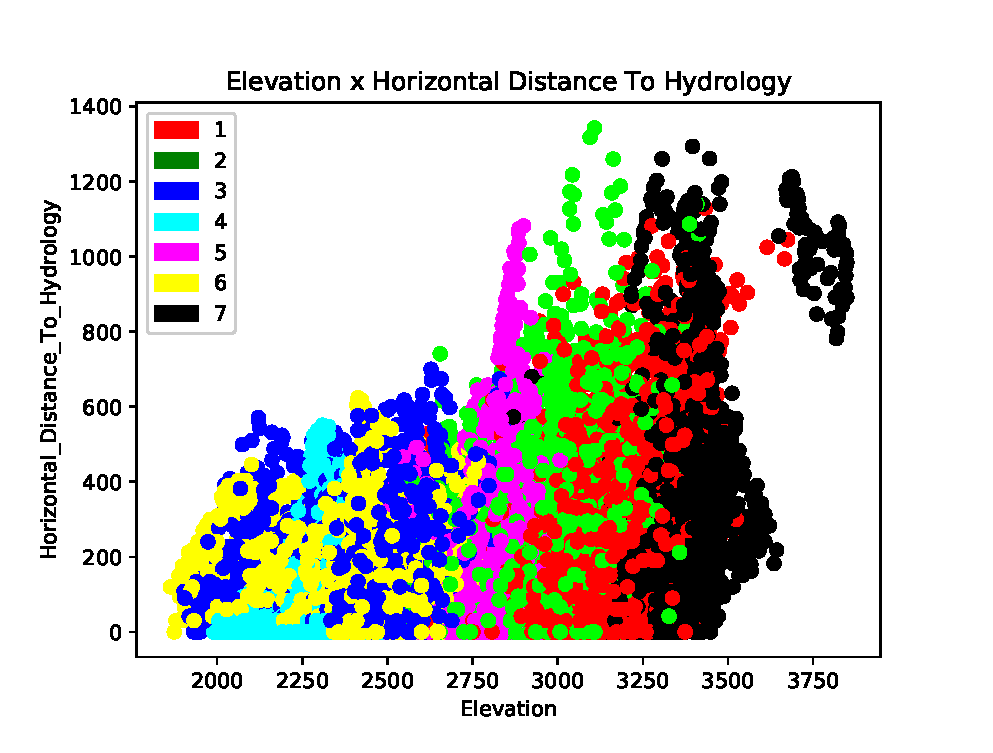
\includegraphics[width=0.5\textwidth]{figs/1.eps}
	}
	\subfloat[]{
		\label{ref:2eps}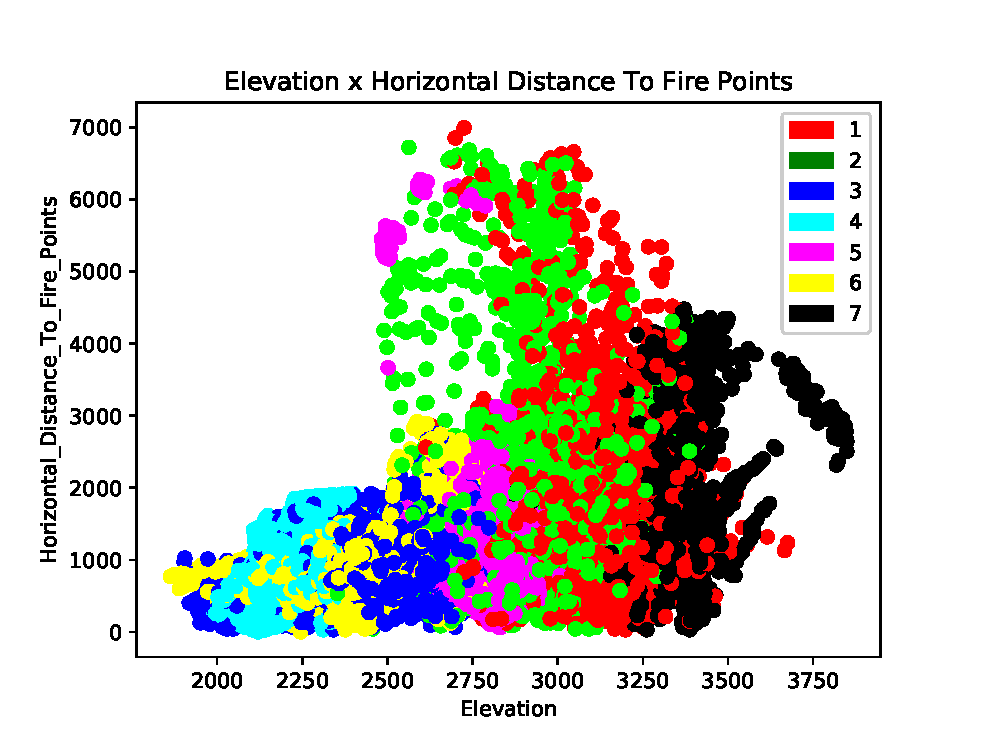
\includegraphics[width=0.5\textwidth]{figs/2.eps}
	}
	\\
	\subfloat[]{
		\label{ref:3eps}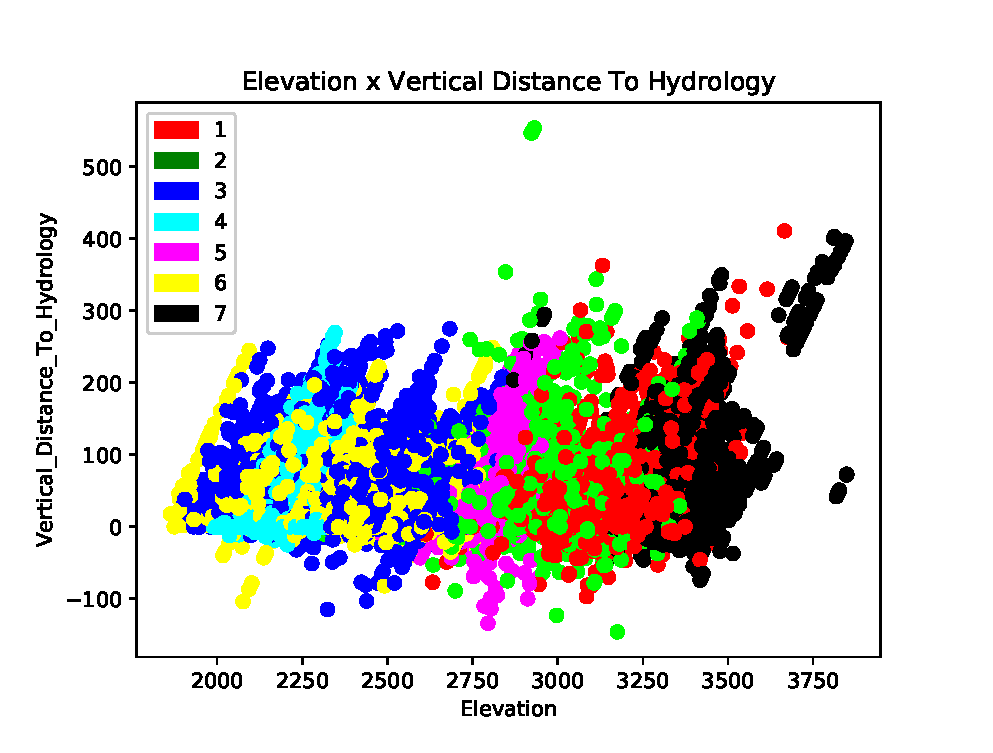
\includegraphics[width=0.5\textwidth]{figs/3.eps}
	}
	\subfloat[]{
		\label{ref:4eps}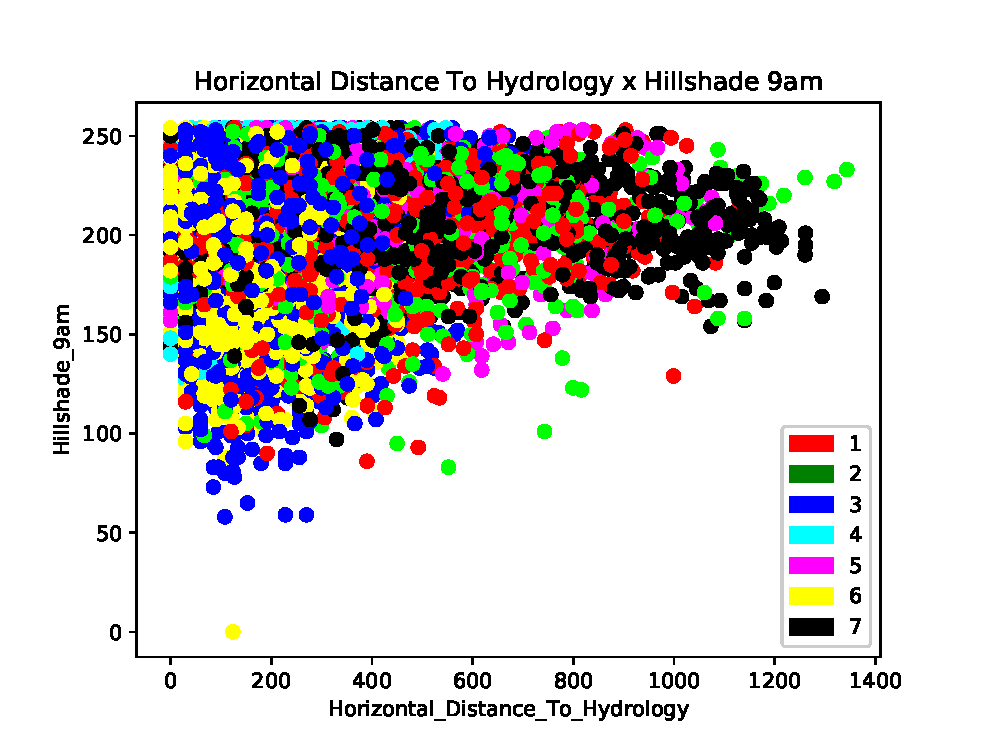
\includegraphics[width=0.5\textwidth]{figs/4.eps}
	}
	\caption{\label{fig:plots}Four examples of dataset's label distribution}
\end{figure}
In \figurename~\ref{fig:plots} we provide four examples of scatter plots based on two features per plot. Figures \ref{ref:1eps}, \ref{ref:2eps} and \ref{ref:3eps}, the labels are well ``separated'', suggesting that some of those features could be a strong candidate to aid classification. Figure \ref{ref:4eps} does not separate as well the different labels, suggesting that the Horizontal distance to hydrology combined (only) with the Hillshade 9am feature are not as good features as the others.